\section{Définition} % 1.1
Le sous-système de communication d'un vaisseau spatial combine la liaison de communication entre le vaisseau spatial et le sol. Des antennes et des émetteurs-récepteurs sont présents à la fois sur le vaisseau spatial et au sol pour transmettre et recevoir des signaux. L'objectif ultime est de garantir une liaison de communication entre le vaisseau spatial et le centre de contrôle de mission pour les phases requises de la mission afin de télécharger des données de charge utile propres et de charger les commandes du vaisseau spatial.

\begin{figure}[H] % H force l'affichage ici
    \centering
    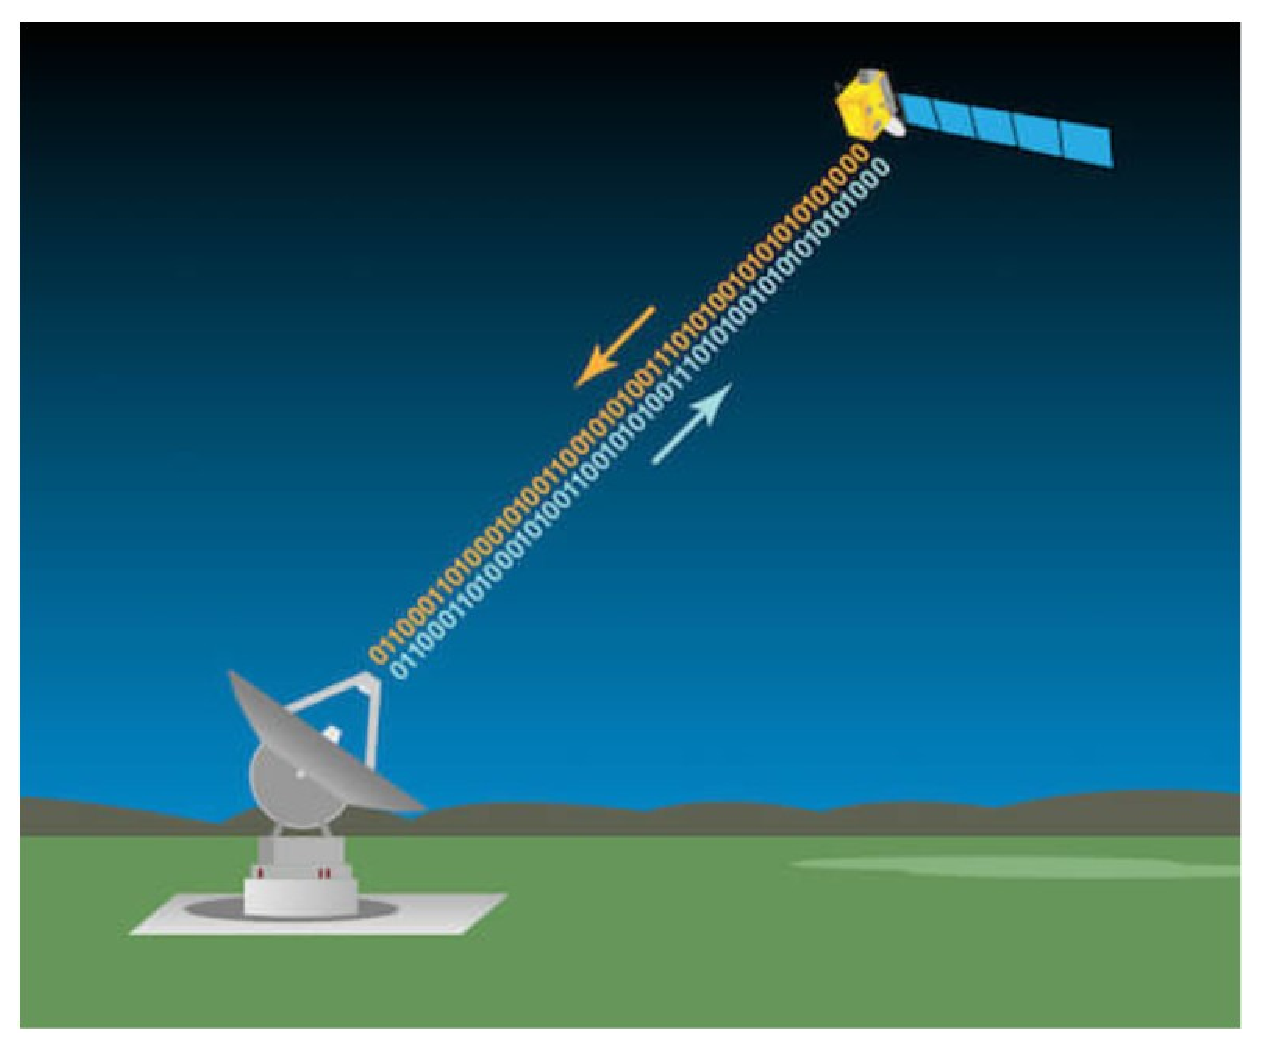
\includegraphics[width=0.5\textwidth]{figures/6-1.eps}
    
    \caption{Illustration d'un vaisseau spatial envoyant et recevant des informations d'une antenne DSN. Crédit image : NASA/JPL-Caltech..}
    \label{fig:communication}
\end{figure}
